\subsection{Introduction}
This secion will go in depth about the extentionboard created as ab addon to the AQ M4 board. The extentionboard was developed to act as a bridge between PC and the CAN-bus using wireless communication in order to send GPS coordinates from the PC to the Drones.\\

The block schematic shown in figure \ref{fig:PCB_block} was created by the auther of the report. It was then given to Carsten Albertsen who created the schematic and did rest of the creation of the PCB.
\\
\Mathias{Create schematic appendix}
\Mathias{Add GPS, WIFI, PCB, PC to forkortelses liste}
\Mathias{Thanks to Carsten Albertsen for PCB development}
\begin{figure}[H]
    \center
    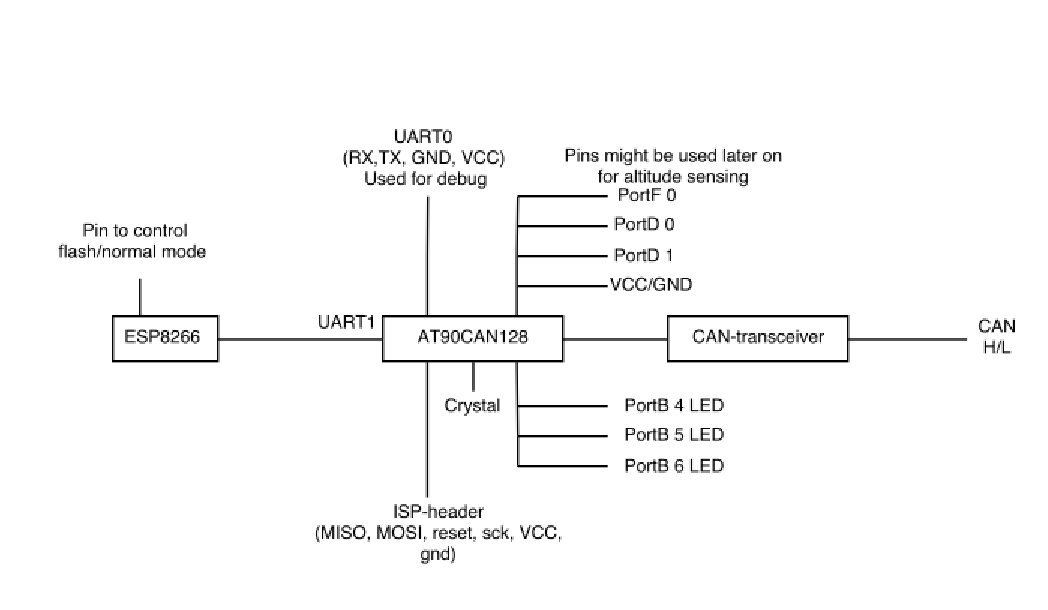
\includegraphics[width=1\textwidth]{graphics/PCB_block_v3.eps}
    \caption{Block schematic of the WIFI-extentionboard developed to AQ M4}
    \label{fig:PCB_block}
\end{figure}

\subsubsection{ATmega}
\subsubsection{Wireless Communication}
An important part of the hardware is the wireless communication used between the PC and the drones.
The wireless communication mpodule has severel requirements it needs to fulfill in order to make the whole system work as expected. A comparesiontable has been made in table \ref{tab:compare_table_wireless_communication} to find the wireless communication module that is best suited for the task.


\begin{table}[H]
	\centering
	\begin{tabular}{@{}|l|l|l|l|l|l|l|@{}}
		\toprule
		\textbf{Product} & \textbf{Size} & \textbf{Price} & 				\textbf{Usability} & \textbf{Power consumption} & 					\textbf{Range} & \textbf{Score} \\ \midrule
		ESP8266          &               &                &                    		&                            &                &                		\\ \midrule
		EMW3165          &               &                &                    		&                            &                &                		\\ \midrule
		nRF51822         &               &                &                    		&                            &                &                		\\ \bottomrule
	\end{tabular}
	\caption{Comparisontable used to compare different wireless 		communication modules}
	\label{tab:compare_table_wireless_communication}
\end{table}

\subsubsection{Pins}
A few pins where made available through solder pads for easy access if needed later on.

The following pins where available as solder pads:
\begin{itemize}
	\item PortF 0 - Alternative function as ADC, channel 0
	\item PortD 0 - Alternative function as interrupt, INT0
	\item PortD 1 - Alternative function as interrupt, INT1
\end{itemize}
In case the onboard baromter isn't accurate enough, an alternative distance could be used to measure the drones altitude with respect to the ground.
PortF0 has been made available since some distance sensors give output as an analogue value. 
An example of such sensor is an Infrared proximity sensor.\footnote{http://www.sharpsma.com/webfm\_send/1208} \\
As an alternative type of distance sensor, a ultrasoinc could be used such as HCSR04.
As output it gives a binary output with high-time proportional with the distance.\footnote{http://www.micropik.com/PDF/HCSR04.pdf}.
To detect the high-time, one of PortD1/0 would be useful. \\

Which type of sensor suits best as a distance sensor to provice altitude information to the drone is ouf of the scope of this report. The PCB has just been made ready to different types of sensors.

\subsubsection{Debug/ISP}
In the final schematic UART0 and ISP pins where combined in one pinheader for easy access through one cable. \Mathias{Refer to image of board}
To program the AtMega the ISP pins where required to be easy accessable. 
UART0 was made accessable to be used as debug and programming of the ESP8266 board.
The plan was to setup the AtMega as UART passthrough from UART0 to UART1.
Due to a mistake\footnote{The wrong pair of MISO/MOSI pins where made available in the ISP-header. The correct pair of MISO/MOSI is also RXD0/TXD0 as alternative function} in the final schematic, both UART0 and UART1 where made accessable trough the ISP/debug header. 
This ended up making it easier to program the ESP8266-board without using the AtMega as UART passthrough.
